\documentclass[12pt,letterpaper]{article}

\usepackage[utf8]{inputenc}
\usepackage[T1]{fontenc}
\usepackage{amsmath}
\usepackage{amsfonts}
\usepackage{amssymb}
\usepackage{amsthm}
\usepackage[left=2cm,right=2cm,top=2cm,bottom=2cm,headheight=22pt]{geometry}
\usepackage{fancyhdr}
\usepackage{setspace}
\usepackage{lastpage}
\usepackage{graphicx}
\usepackage{caption}
\usepackage{subcaption}
\usepackage{paralist}
\usepackage{url}

\theoremstyle{definition}
\newtheorem{question}{Question}
\newtheorem{example}{Example}
\newtheorem{exercise}[question]{Exercise}
\newtheorem*{challenge}{Challenge}
\newtheorem*{theorem}{Theorem}
\newtheorem*{definition}{Definition}

\begin{document}

%Paramètres de mise en forme des paragraphes selon les normes françaises
\setlength{\parskip}{1ex plus 0.5ex minus 0.2ex}
\setlength{\parindent}{0pt}

%Paramètres relatifs aux en-têtes et pieds de page.
\pagestyle{fancy}
\lhead{Theron J Hitchman}
\chead{\Large Reading and Guided Practice \#01}
\rhead{Spring 2016}
\lfoot{\emph{Math and Decision Making }}
\cfoot{}
\rfoot{\emph{\thepage\ of \pageref{LastPage}}}

\section*{Introduction}
In this assignment, you will learn about the basics of \emph{Graph Theory}  through two easy-to-state puzzles
about connecting ``things.''

\section*{Goals}
At the end of this assignment, a student should be able to:
\begin{compactitem}
\item Describe what a graph is clearly.
\item Use the terms \emph{vertex} and \emph{edge} properly.
\item Describe what the crossing number of a graph is.
\end{compactitem}
A student might also be able to:
\begin{compactitem}
\item Translate problems about different kinds of networks into graph theory terms.
\end{compactitem}

\section*{Reading and Questions for Graph Theory Meeting Two}

\subsection*{A Puzzle about Roads}

Imagine you are planning a brand new civilization on a vast plain. (If you want, you can imagine it on a vast plane. 
Sorry. I can't help the math jokes.) Because you are planning from scratch, you can place the cities wherever you like, 
and you can choose how to join those cities with highways.   To make sure everything is connected up, you want to design things so that each of your cities is connected to each of 
the other cities by a designated highway. So, if we decide on three cities named Davidopolis, Juliaburgh, and Penelopeville, we will want enough highways that there is one joining Davidopolis to Juliaburgh, one joining Davidopolis to Penlopeville, and one joining Juliaburgh to Penelopeville. That's three roads.

\begin{figure}[h]
\centering
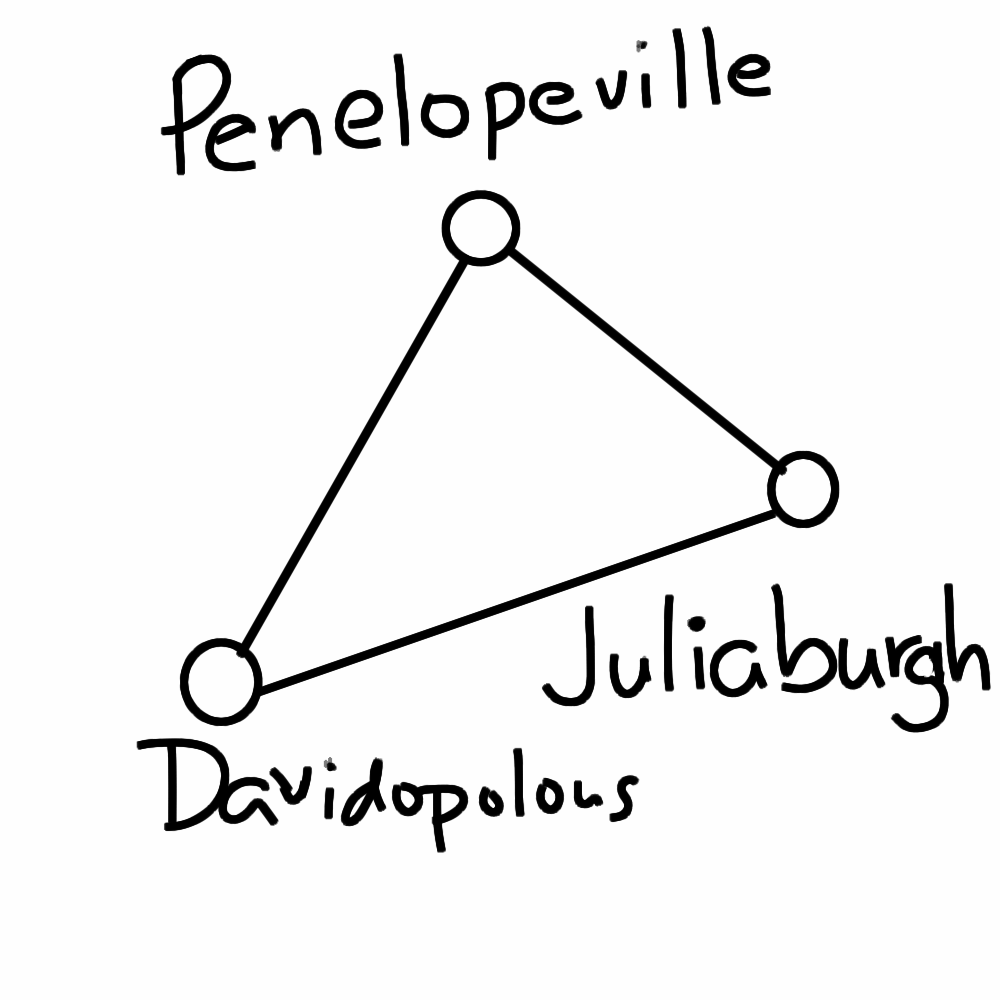
\includegraphics[width=.4\textwidth]{images/ThreeTowns.png}
\caption{A Map with Three Randomly Named Towns}
\end{figure}


\subsection*{Abstraction as a verb}

An important thing has already happened, and we haven't even stated the puzzle, yet.  Note that I decided to represent cities with dots on the page, and roads with lines joining those dots. I DID NOT actually build a bunch of cities and roads to see how things would turn out. That would be too expensive and time-consuming. (I don't even know
how to weld.)

These dots and lines are \emph{abstractions}. We have taken away lots of detail that we don't need, like buildings and people, and left only the parts we do need: some places and some things which join the places. The process of making abstractions is a crucial bit of how mathematics gets done. You probably do it all the time without even noticing. We will want to do it often.

\subsection*{An Example}

Now let's make a set-up with five cities. If we draw one of our abstract representations, we need five little nodes,
and one line for each pair of nodes. If you count carefully, that makes ten lines. Take a second and draw that. 
Your picture should look something like this one:

\begin{figure}[h]
\centering
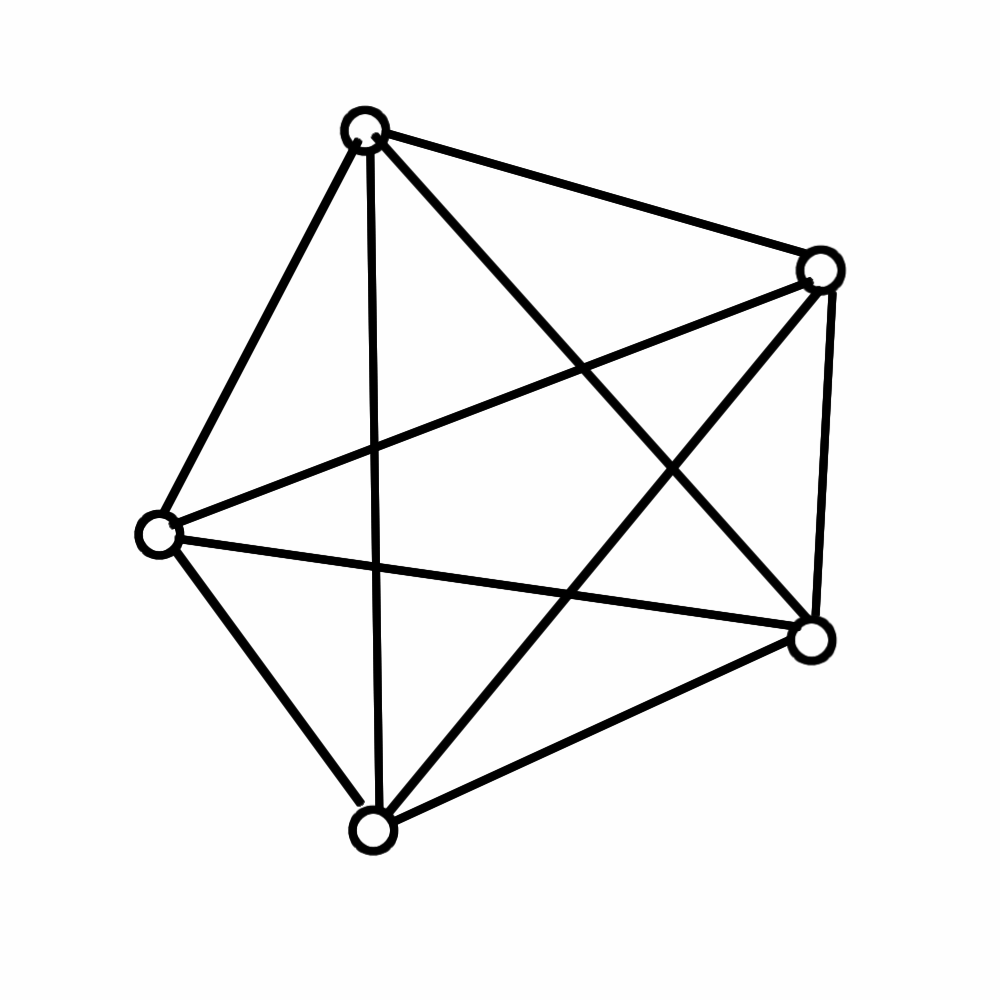
\includegraphics[width=.5\textwidth]{images/k5.png}
\caption{The Complete Graph on Five Vertices}
\end{figure}

Our two pictures so far are examples of things called \emph{graphs}. Mathematicians have been studying these
for a few hundred years, now, and the subject is called \emph{graph theory}. There is a formal definition, but for 
now, it is enough to know that a graph consists of a bunch of things which are our nodes, and called 
\emph{vertices}, and a bunch of connectors between those nodes, called \emph{edges}.  By the way, the singular of \emph{vertices} is \emph{vertex}. 

The star-in-a-pentagon picture above is called the \emph{complete graph} on five vertices. It is complete because every pair of vertices has an edge in the graph which joins them.

\begin{exercise}
Draw the complete graph on three vertices. Have you seen this graph before?
\end{exercise}

\begin{exercise}
Draw the complete graph on four vertices.
\end{exercise}

\begin{exercise}
Draw a graph with five vertices which is different from the complete graph on five vertices. By ``different,'' I mean that the graph should represent a different set of logical relationships between five things.
\end{exercise}

\subsection*{The Puzzle, Finally}

I said we would play with a puzzle or two, right? Here is the first one.

It depends on the idea that when two roads cross, you have to build an intersection or an overpass. Those are expensive, and we want to avoid them.

\begin{quotation}\textbf{The Five Cities Puzzle:} Layout a plan for five cities with a road joining each pair of cities in such a way that none of the roads cross.
\end{quotation}

\begin{challenge}
Find a solution to the Five Cities Puzzle.
\end{challenge}

I have a suggestion at this point. The Five Cities Puzzle is a challenging one. You might get frustrated and feel stuck.
But here is some general problem-solving advice from a famous teacher named George Polya:

\begin{quotation} If you are having trouble, find a simpler problem and solve it. 
\end{quotation}

In this case, you \textbf{can} make your problem simpler (how?) and solve the simpler puzzle. Does that help you
solve the Five Cities Puzzle?

\subsection*{Another Puzzle: Three Utilities}

Let's try another puzzle. It is related, as I am sure you will see. This time, I will leave the whole thing to you. All of the abstraction, all of the drawing, all of the thinking.

\begin{quotation}\textbf{Three Utilities Puzzle} A certain town has three houses in it and three utilities: water, 
electricity, and internet. We wish to connect each of the houses to each of the utilities with its own dedicated service 
line, which is to be buried. But it is dangerous to bury one line across another, as you might get injured if you accidentally cut a line. 

Design a layout that allows each of the houses to be connected to each of the utilities so that no service lines cross.
\end{quotation}

\begin{challenge}
Solve the Three Utilities Puzzle.
\end{challenge}

\begin{exercise}
Make a simpler version of the Three Utilities Puzzle and solve that instead. How many variants can you think of? How many of those can you solve?
\end{exercise}


\clearpage

\subsection*{A Last Bit of Abstraction}

The puzzles you have tried to solve all boil down to thinking about drawing graphs on paper in such a way that their
edges never cross. I should tell you that for some graphs this is impossible. Sad but true. If instead we made the graphs in 3-dimensional space, so that we could vary the heights of things, then there would be no problem. But our puzzles ask us to draw certain graphs on paper. This is where the challenge comes from.

A funny thing that mathematicians often do is to make up a number that helps \emph{measure failure} of 
something they wanted. In this case, we wanted no crossings. Well, if a graph forces us to have a crossing, so be it.
But we can still ask, ``How many crossings do I need? How few can I get away with?"

\begin{definition}
Let $G$ be a graph. The smallest number of crossings of edges required to draw a representation of the graph on a piece of paper is called the \emph{crossing number} of $G$. Sometimes, people write $\mathrm{cr}(G)$ to stand for the crossing number of $G$.
\end{definition}

\begin{exercise}
Show that the crossing number of the complete graph on three vertices is zero.
\end{exercise}

\begin{exercise}
Show that the crossing number of the complete graph on four vertices is zero.
\end{exercise}

\begin{exercise}
Restate the Five Cities Puzzle in a way that correctly uses the concept of crossing number.
\end{exercise}

\begin{challenge}
Make an example of a graph for which you are \emph{certain} the crossing number is not zero.
Be sure to write down your argument for why it can't be zero.
\end{challenge}



%\begin{thebibliography}{9}
%\end{thebibliography}

\end{document}
%sagemathcloud={"zoom_width":100}